% Please make sure you insert your
% data according to the instructions in PoSauthmanual.pdf
\documentclass[a4paper,11pt]{article}
\usepackage{pos}

\title{Comparison of Kerr and dilaton black hole shadows}
\ShortTitle{Comparison of Kerr and dilaton black hole shadows}

\author*[a]{Jan Röder}
\author[a]{A. Cruz-Osorio}
\author[a]{C. M. Fromm}
\author[a,b]{Y. Mizuno}
\author[c,d]{Z. Younsi}
\author[a,e,f]{L. Rezzolla}


\affiliation[a]{Institut f\"ur Theoretische Physik,\\ Max-von-Laue-Stra{\ss}e 1, D-60438 Frankfurt am Main, Germany}

\affiliation[b]{Tsung-Dao Lee Institute and School of Physics and Astronomy,\\ Shanghai Jiao Tong University, Shanghai, 200240, China}

\affiliation[c]{Mullard Space Science Laboratory,\\ University College London, Holmbury St. Mary, Dorking, Surrey, RH5 6NT, UK}

\affiliation[d]{UKRI Stephen Hawking Fellow}

\affiliation[e]{Frankfurt Institute for Advanced Studies,\\ Ruth-Moufang-Stra{\ss}e 1, 60438 Frankfurt am Main, Germany}

\affiliation[f]{School of Mathematics, \\ 
Trinity College, Dublin 2, Ireland}


\emailAdd{jroeder@itp.uni-frankfurt.de}
\emailAdd{osorio@itp.uni-frankfurt.de}
\emailAdd{cfromm@itp.uni-frankfurt.de}
\emailAdd{mizuno@itp.uni-frankfurt.de}
\emailAdd{z.younsi@ucl.ac.uk}
\emailAdd{rezzolla@itp.uni-frankfurt.de}


\abstract{
The vicinity of supermassive black holes (SMBHs) has been in the focus of scientific research for decades. Open questions revolve around the types of compact objects in the centers of galaxies, plasma dynamics around them and emission processes at play. The goal of this study is to assess whether it is possible to distinguish between two spacetimes in observations by means of synthetic imaging. %, under the aspect of different emission models. 
To this end, general relativistic radiative transfer (GRRT) calculations are carried out on general relativistic magneto-hydrodynamics (GRMHD) simulations of a Kerr and of a non-rotating dilaton black hole. We parametrize the proton-to-electron temperature ratio and analyze the source morphology.


%and further generate synthetic VLBI data that images are reconstructed from. 

% Extending the studies conducted in the pioneering work of Mizuno \textit{et al.} 2018,  
 
% The systems are matched at the innermost stable circular orbit, and both black holes are initially surrounded by a torus in hydrostatic equilibrium with a weak poloidal magnetic field. 
 
% In order to investigate the plasma dynamics, GRMHD simulations were carried out using the ``Black Hole Accretion Code'' (BHAC). 
 
% In the literature the ratio between the temperatures of simulated ions and radiating electrons is often taken to be a constant, while in reality it is expected to depend on plasma properties. 
 
% In radiative post-processing with the code ``Black Hole Observations in Stationary Spacetimes'' (BHOSS) the temperature ratio was therefore parametrized. 
 
% Additionally, in the jet wall, electrons are believed to be accelerated and should therefore be modeled with non-thermal electrons. To this end, both thermal and non-thermal electron energy distribution functions were employed. 
 
% Lastly, images were reconstructed from synthetic VLBI data with the ``eht-imaging'' Python package to study how the effects of the emission models carry over to an observational environment. 
 
% The most impactful result is the effect of the parameter $R_{\rm high}$ in the temperature ratio parametrization, splitting source structures into torus-- and jet dominated configurations. 
 
% Non-thermal emission turns out to be negligible at the field of view used and for the region it is applied in. 
 
% Hence, given the present observational capabilities, it is unlikely that it is possible to distinguish spacetimes in observations. The striking visual differences are due to the difference in rotation between the black holes. 
 
% In synthetic VLBI images, even the difference in shadow size is lost for most configurations. The situation may be improved in the future by a better VLBI array.
}

\FullConference{%
  *** European VLBI Network Mini-Symposium and Users' Meeting (EVN2021) ***\\
  *** 12-14 July, 2021 ***\\
  *** Online ***
}

%% \tableofcontents

\begin{document}
\maketitle

\section{Introduction}

Ever since the discovery of quasars in the early 1960, studies of active galactic nuclei (AGN) have been a prominent field in astronomy \cite{Shields1999}. Soon, black holes were generally accepted as the root of the observed extreme-energy output of some galaxies. Over the decades, evidence for the existence of (supermassive) black holes was first found indirectly through movement of stars in the galactic center \cite{Eckart1996,Ghez1998} and the first detection of gravitational waves \cite{Abbott2016a}. Most recently, the Event Horizon Telescope Collaboration obtained a direct image of the shadow of the SMBH at the heart of M\,87 \cite{EHT_M87_PaperI}. \\
Ever since it was first published \cite{Einstein1916}, Einstein's theory of general relativity has been put to the test countless times. Putting our own spin on the ongoing debate on general relativity, the goal of this work is to assess whether a Kerr black hole can be distinguished from a dilaton black hole by means of magnet-hydrodynamic modeling in full general relativity and subsequent radiative post-processing.

\section{Methods}
\subsection{General-Relativistic Magneto-hydrodynamics (GRMHD)}
Following the pioneering work of Mizuno et al. 2018 \cite{Mizuno2018}, we choose as representative systems a Kerr black hole with dimensionless spin $a_\star=0.6$ and a non-rotating dilaton black hole with dilaton parameter $b=0.504$ in spherically symmetric polar coordinates. The latter black hole is described by the Einstein-Maxwell-dilaton-axion (EMDA) gravity \cite{Garcia1995}, with the axion field set to zero. The two black holes are matched at the innermost stable circular orbit (ISCO). \\

The GRMHD equations consisting of local conservation of mass, energy and momentum along with Faraday's law read \cite{Rezzolla_book:2013,Porth2017}:
\begin{align} 
\nabla_\mu\left(\rho u^\mu\right)=0,\ \ \ \nabla_\mu T^{\mu\nu}=0,\ \ \ \nabla_\mu {}^{*}\!F^{\mu\nu}=0,\label{eq:grmhd_eqs}\\
T^{\mu\nu}=\rho h_{\rm tot}u^\mu u^\nu +p_{\rm tot} g^{\mu\nu}-b^\mu b^\nu,\label{eq:Tmunu}\\
 ^{*}\!F^{\mu\nu}=b^\mu u^\nu - b^\nu u^\mu,\label{eq:Fmunu}
\end{align}
In Eq. \ref{eq:grmhd_eqs}, $\rho$ is the rest mass density and $u^\mu$ is the fluid four-velocity. Equations \ref{eq:Tmunu} and \ref{eq:Fmunu} show the energy-momentum tensor $T^{\mu\nu}$ and the dual of the Faraday tensor $^{*}\!F^{\mu\nu}$, with total pressure $p_{\rm tot}=p+b^2/2$ and specific enthalpy $h_{\rm tot}=h+b^2/\rho$. Lastly, $b^2=b^\mu b_\mu$ and $b^\mu$ describe the magnetic field strength in the fluid frame and magnetic field four-vector. \\ 
Both GRMHD simulations are initialized with a static hydrostatic equilibrium torus with a constant angular momentum distribution \cite{Font02b,Rezzolla_book:2013}. The torus is governed by an ideal gas equation of state with adiabatic index $\Gamma=4/3$, while on the outside pressure and density floor values are applied \cite{Mizuno2018}. The gas pressure in the torus is perturbed by 1\% in order to trigger the magneto-rotational instability, which starts and drives the accretion of gas onto the black hole. \\
We add a poloidal magnetic field onto the constructed torus, with the vector potential in the form $A_\phi \propto \max\left(\rho/\rho_{\rm max}-0.2,0\right)$.
%\begin{equation}
%A_\phi \propto \max\left(\rho/\rho_{\rm max}-0.2,0\right).
%\end{equation}
This magnetic field configuration will produce a Standard and Normal Evolution (SANE) \cite{Narayan2012,Mizuno2018,Ripperda2020} of both black hole systems. Specifications of the GRMHD grid and fluid parameters are summed up in table \ref{tab:grmhd_params}.
\begin{table}[h!]
	\vspace{-0pt}
	\centering
	\caption{GRMHD simulation parameters, adapted from \cite{Mizuno2018}. $r_{\rm eh}$ is the event horizon radius.}
	\begin{tabular}{llll} 
		\hline \hline
		
		\multicolumn{4}{c}{Plasma parameters}\\
		adiab. index $\Gamma$ & density floor $\rho_{\rm fl}$ & pressure floor $p_{\rm gas,\ fl}$  & \\
		\hline
		$4/3$ & $10^{-4} r^{-3/2}$ &$ (10^{-6}/3) r^{-5/2}$ &\\
		\hline 		
		
		
		\multicolumn{4}{c}{Grid extent}\\
		radial, $r$ & azimuthal, $\theta$ & polar, $\phi$ & cells, $(N_r,N_\theta,N_\phi)$\\
		\hline
		$ \left(0.8\,r_{\rm eh}, 1,000\,{\rm M}\right)$ &$ \left(0.01\pi, 0.99\pi\right)$ &$\left(0, 2\pi\right) $&$\left(256,128,128\right)$ \\
		\hline 
		
		
		\multicolumn{4}{c}{Other parameters$^\ast$}\\
		 $a$ & $b$ & $l_{\rm torus,\ Kerr}$ & $l_{\rm torus,\ dilaton}$ \\
		\hline 
		$0.6$ & $0.504$ & $4.5$ & $4.567$ \\
		\hline 
		
		\multicolumn{4}{l}{$^\ast$ Kerr dimensionless spin parameter, dilaton parameter and specific angular momenta} \\
		\label{tab:grmhd_params}
	\end{tabular} 
%	\vspace{-12pt} 
\end{table} 
The GRMHD simulations are carried out using the \texttt{Black Hole Accretion Code BHAC} \cite{Porth2017} in modified Kerr-Schild coordinates. The GRMHD equations are evolved in a finite-volume representation. At each time step, we employ a piecewise-parabolic method, a total variation diminishing Lax-Friedrichs theme amd a predictor-corrector scheme to update the fluid variables \cite{Porth2017}. %dilaton in RZ param?
Further, the condition $\boldsymbol{\nabla B} =0$ is handled by flux-interpolated constrained transport (FCT) \cite{Porth2017}. 


\subsection{General-Relativistic Radiative Transfer (GRRT)}

We model synchrotron emission by carrying out GRRT calculations on the GRMHD simulations. Making use of the fast-light approximation, light rays (null geodesics) are integrated from a far-away observer to the black hole system. Subsequently, the intensity and optical depth equations are solved along each light ray \cite{Younsi2012}. Between 11,\,000\,M and 12\,000\,M of the GRMHD simulations, 101 snapshots images are generated. The mass accretion rate is fixed at the 10\,000\,M snapshot to yield a flux of 3\,Jy at 230\,GHz. \\
The GRRT calculations are carried out with the \texttt{Black Hole Observations in Stationary Spacetimes BHOSS} code (Younsi et al. (2021), in prep.). A Runge-Kutta-Fehlberg integrator handles the light rays, whereas the intensity and optical depth are simply updated in an Eulerian scheme. The far-away observer is a plane perpendicular to the line of sight. For further details, see \cite{Younsi2016}. All GRRT calculation parameters are collected in table \ref{tab:grrt_params}.  
\begin{table}[h!]
	\vspace{-0pt}
	\centering
	\caption{GRRT calculation parameters}
	\begin{tabular}{lllll} 
		\hline \hline
		
		\multicolumn{5}{c}{Imaging}\\
		No. of pixels & ${\rm width}/r_g$  & ${\rm width}/\upmu$as& inclination & Target flux\\
		\hline
		1024\,$\times$\,1024 & $40\times40$ & $211\times211$ &60$^\circ$ &3\,Jy\\
		\hline 		
		
		\multicolumn{5}{c}{Emission}\\
		&$R_{\rm low}$ & $R_{\rm high}$& eDF \\
		\hline
		&1& 10, 80, 160 & thermal \\
		\hline 		

		%\multicolumn{5}{l}{$^\ast$ Kerr dimensionless spin parameter, Dilaton parameter and specific angular momenta} \\
		\label{tab:grrt_params}
	\end{tabular} 
	%	\vspace{-12pt} 
\end{table} 
Since in the vicinity of black holes in active galactic nuclei various heating processes lead to different temperatures of electrons and protons, we relate the radiating electrons to the simulated protons by the "R-$\beta$-parametrization" (\cite{Moscibrodzka2016}; see also \cite{Cruz-Osorio2021,Fromm2021b,Davelaar2019}):
\begin{equation} \label{eq:tratio_beta}
\frac{T_{\rm p}}{T_{\rm e}}=\frac{R_{\rm high}\,\beta^2+R_{\rm low}}{1+\beta^2}\,.
\end{equation}
In the above equation, $\beta\equiv p_{\rm\,gas}/p_{\rm\,mag}$ is the ratio of gas-- to magnetic pressure. The parameters $R_{\rm high}$ and $R_{\rm low}$ control the temperature ratio in regions where $\beta\gg1$ (the disk) and $\beta\ll1$ (the jet), respectively. We set the synchrotron emission to be purely thermal. The corresponding electron distribution function reads \cite{Leung2011}:
\begin{equation}\label{eq:rel_thermal}
\frac{dn_{\rm e}}{d\gamma_{\rm e}\,d\cos\xi\,d\phi} = \frac{n_{\rm e}}{4 \pi \Theta_{\rm e}} \frac{\gamma_{\rm e} \left(\gamma_{\rm e}^2 - 1\right)^{1/2}}{K_2\left(1/\Theta_{\rm e}\right)} \exp \left(- \frac{\gamma_{\rm e}}{\Theta_{\rm e}}\right),
\end{equation}
with electron number density $n_{\rm e}$, gyrophase $\phi$, Lorentz factor $\gamma_{\rm e}$, pitch angle $\xi$ and modified Bessel function of the second kind $K_2$. Absorptivities and emissivities are taken from \cite{Pandya2016}. 


\section{Results}

The GRMHD simulations of the Kerr- and dilaton black holes enter a relaxed state past 10\,000\,M and show very similar overall behavior. This was to be expected, since the two systems were matched at their ISCO. While the code accretion rates in the Kerr system are only slightly higher, the normalized magnetic flux through the horizon is doubled compared to the dilaton case. We define in the following the jet sheath as $0.1\leq\sigma\leq1.0 \wedge Be\geq1.02$, where $Be=-h\,u_t$ is the Bernoulli parameter. Lower magnetized regions we identify with the torus.\\
Both black hole systems show an overall intermediate to low magnetized torus, where $\sigma \lesssim 10^{-2}$. In contrast to the dilaton black hole, the Kerr system shows a highly magnetized jet with a wider opening angle. This is due to more magnetic flux piling up near the horizon, caused by the Kerr black hole's rotation.\\
As mentioned above, employing the R-$\beta$-parametrization leaves the (dimensionless) electron temperature $\Theta_{\rm e}$ in the jet unaltered, whereas an increase of $R_{\rm high}$ leads to a decrease of electron temperature in the torus. For example, at $R_{\rm high}=10$ electrons in the torus are hot ($\Theta_{\rm e}\sim 2.5$), and much cooler for $R_{\rm high}=160$ ($\Theta_{\rm e}\sim0.1$).\\

\begin{figure}[h!]
	\centering
	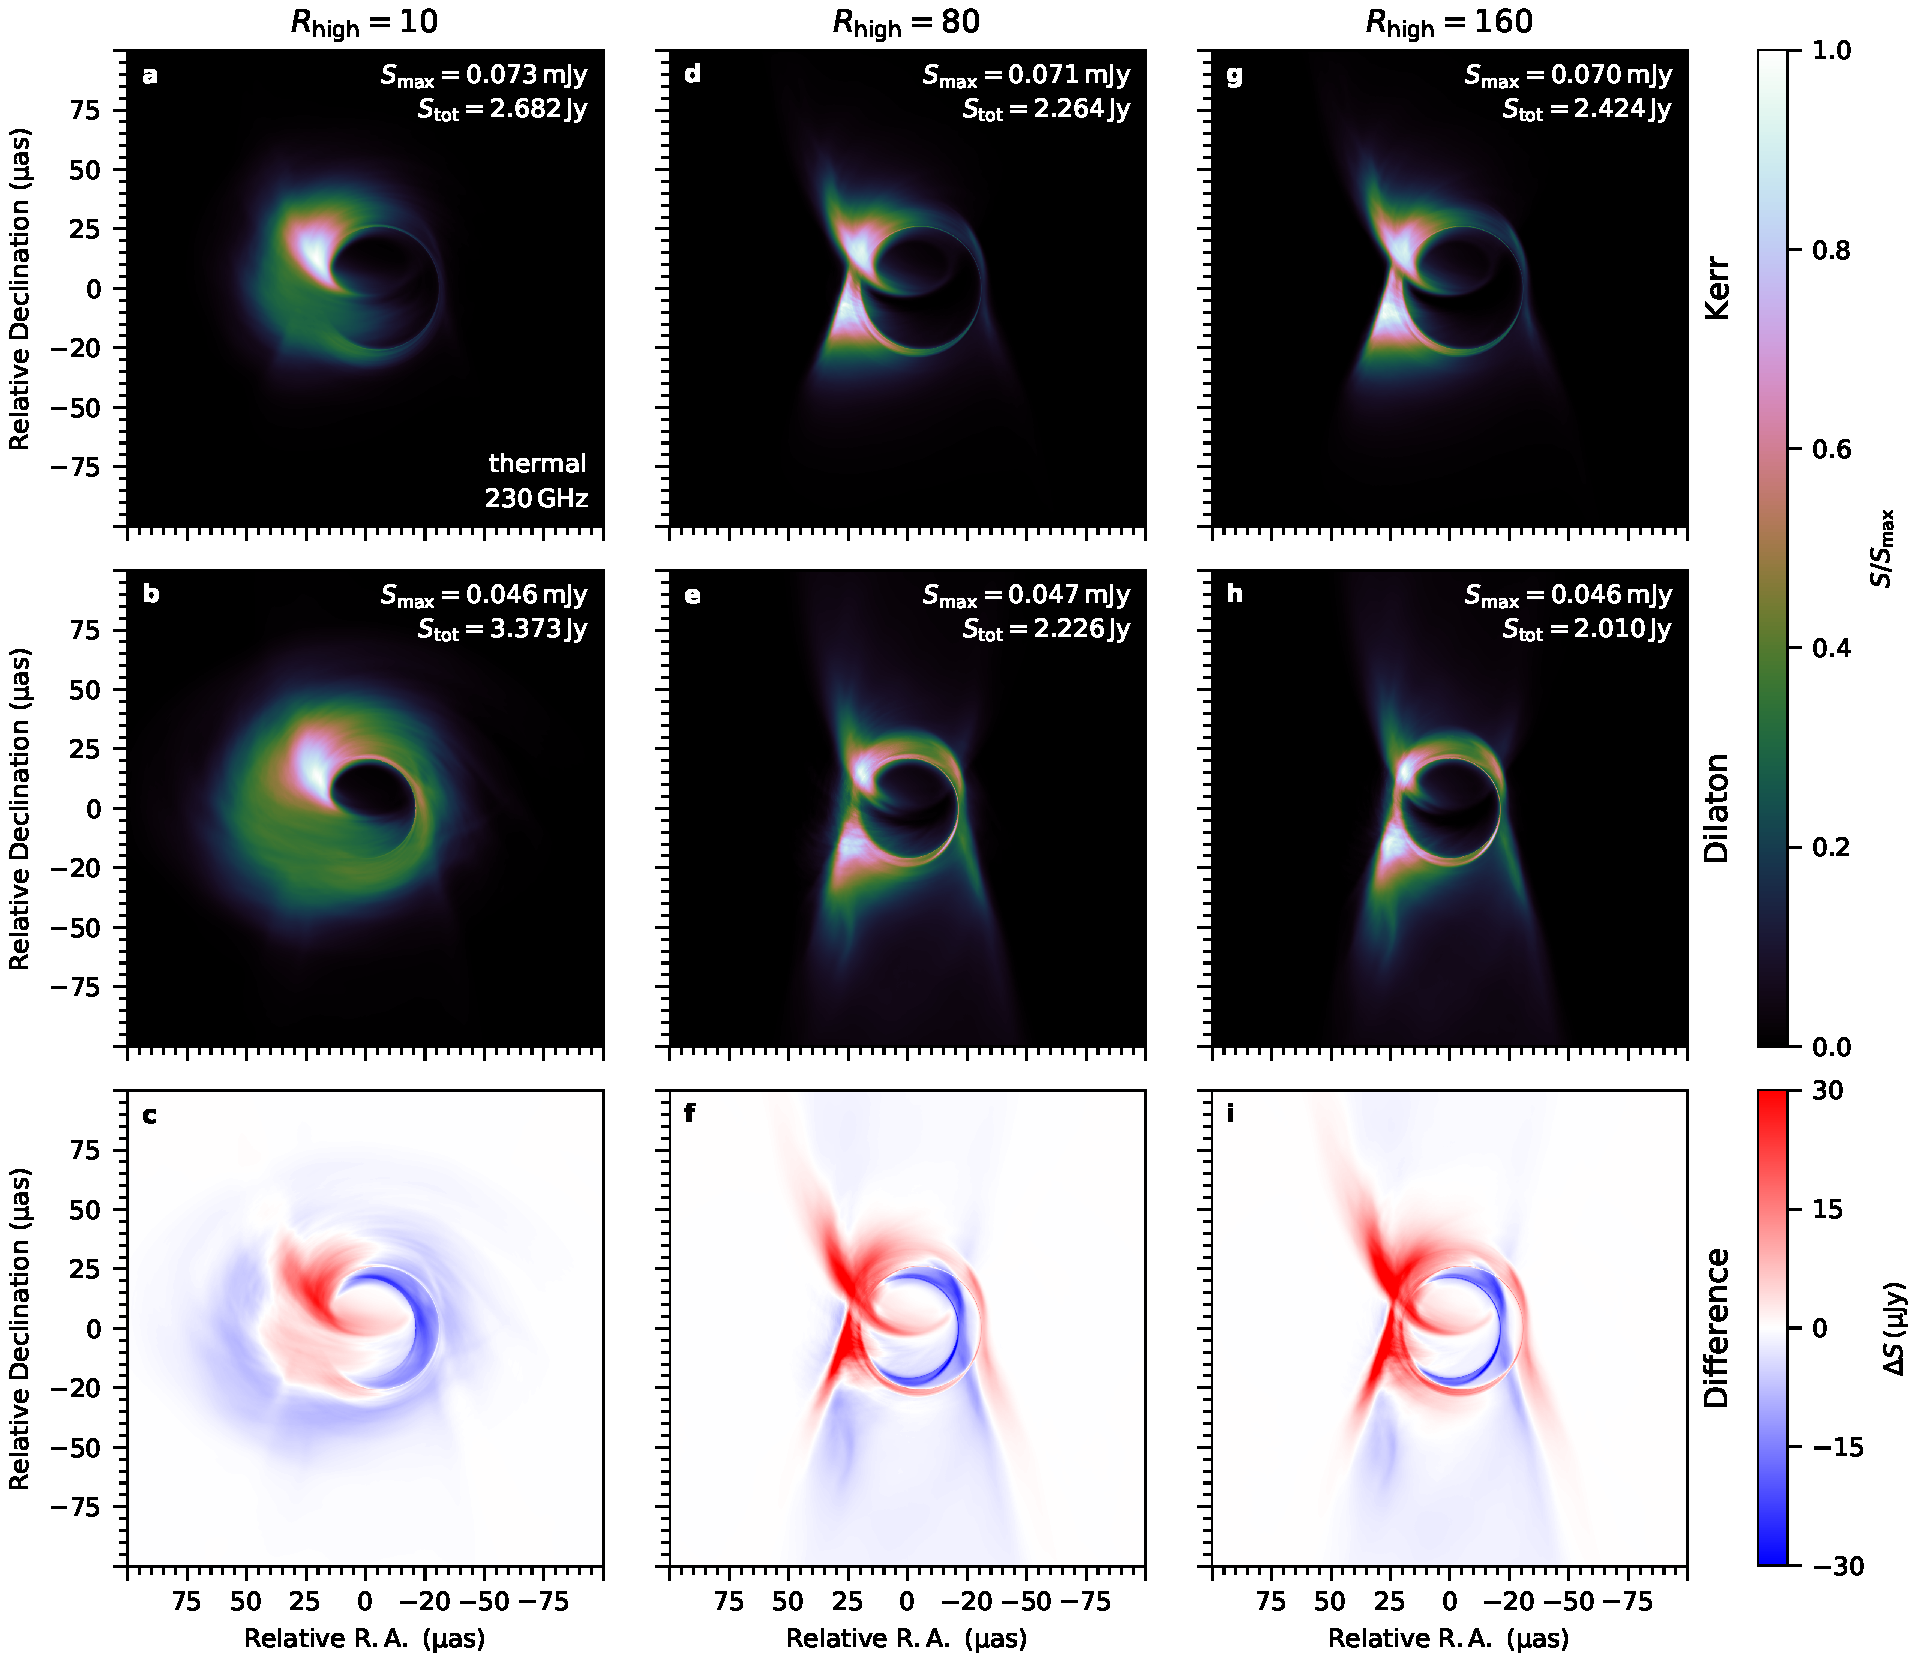
\includegraphics[width=\textwidth]{proc_SgrA_SANE_a06_230GHz_Rh1_i60_ovpl.pdf}
	\caption{Effect of the $R(\beta)$ parametrization on averaged GRRT images of a Kerr black hole (top row) and a dilaton black hole (middle row), along with pixel-by-pixel differences (bottom row). Images are generated with thermal synchrotron radiation at 230\,GHz and averaged over 101 snapshots taken between 11,\,000\,M to 12,\,000\,M of the GRMHD simulation.}
	\label{fig:GRRT}
\end{figure} 

Figure \ref{fig:GRRT} shows averaged GRRT images for three values of $R_{\rm high}$, along with pixel-by-pixel differences between Kerr- and dilaton black holes of the same emission model. The resulting total flux varies among models since we did not fix the total flux for the average image, but for a single snapshot. The R-$\beta$-parametrization essentially divides all GRRT images in torus-dominated ($R_{\rm high}=10$) and jet-dominated ($R_{\rm high}>10$) models. The torus in the former class of models extends further inward and outward for the dilaton black hole. On the one hand, there is more distance to cover for accreted matter. This is due to the smaller event horizon of the dilaton black hole caused by the ISCO matching. On the other hand, increased Doppler beaming around the Kerr black hole leads to significant differences in the brightness distributions between the spacetimes in the torus-dominated configurations (see panels a and e of Fig. \ref{fig:GRRT}).\\
In the Kerr image (panel a), the approaching limb is very prominent, while the receding limb is still barely visible at all. The region around the point of peak flux north-west of the shadow shows a sharp boundary past 60\,\% of the peak. The adjacent lower-flux region merges into an arc of emission from the torus and the jet foot-point spanning halfway across the Kerr shadow. South-west of the shadow, the faint onset of the counter-jet is visible. In the dilaton spacetime, the receding limb is much more apparent, and the aforementioned 60\,\% flux region is not as clearly cut as in the Kerr system.\\
The pixel-by-pixel differences again highlight prominent Doppler boosted emission on the approaching side of the Kerr system especially close to the shadow, while the dilaton system exhibits filamentary structures from $\sim$\,30\,$\upmu$as from the center outwards.\\

For $R_{\rm high}=80$, the source structure changes fundamentally from a torus-dominated system towards a jet onset extending outwards into filaments (middle column of figure \ref{fig:GRRT}), showing the wider opening angle in the Kerr system. For both spacetimes, the most of the emission comes from two ``hot-spots'' located at the northern and southern halves of the approaching side close to the shadow. Overall, the source structures of Kerr- and dilaton images are much more similar than for low $R_{\rm high}$. The arc of emission discussed above reduces to the part that traces the foot of the observer-facing jet. Pixel-by-pixel differences (panels f and i) further illustrate the filamentary structures and show how the effects of Doppler boosting affect both the region close to the shadow and the jet onset.\\
Increasing $R_{\rm high}$ to 160, the source structure remains unaltered (rightmost column of figure \ref{fig:GRRT}); the electron temperature in the torus at $R_{\rm high}=80$ is already too low for an additional decrease to make a noticeable difference in the images.


\section{Summary and Conclusion}

In this work, we carried out GRRT calculations on GRMHD simulations of a Kerr- and a dilaton black hole, employing a parametrization for the electron temperature. For each emission model, we compare the images between the two spacetimes. \\
The black hole shadows are clearly distinguishable, since the event horizons of the two black holes are of different sizes due to the ISCO match. The Kerr shadow is asymmetric and off-centered, while the the dilaton shadow is circular and smaller. The R-$\beta$-parametrization splits the source morphologies into torus- and jet dominated images, where the former show the largest differences between spacetimes. Mainly, the torus is more prominent in the dilaton system due to the reduced Doppler boosting compared to the Kerr case. The jet on the other hand shows a larger opening angle and higher magnetization in the Kerr system.\\

Clearly, GRRT calculations lead to infinite-resolution images not reflecting a real-world observing scenario. In order to assess whether Kerr- and dilaton black holes can be distinguished in an actual observation, synthetic VLBI data has to be generated from the GRRT images, mimicking an observation campaign. Further, we expect electrons in the jet to be accelerated by magnetic reconnection, requiring the use of a non-thermal electron energy distribution function during the GRRT calculations. Both of these aspects will play a key role in Röder et al. 2021 (in preparation). 




\bibliographystyle{JHEP}
\bibliography{aeireferences_use.bib}

\end{document}
